% This is a Basic Assignment Paper but with like Code and stuff allowed in it, there is also url, hyperlinks from contents included. 

\documentclass[openany]{report}

% Preamble

\usepackage[margin=1in]{geometry}
\usepackage{amsfonts, amsmath, amssymb}
\usepackage{fancyhdr, float, graphicx}
\usepackage[utf8]{inputenc} % Required for inputting international characters
\usepackage[T1]{fontenc} % Output font encoding for international characters
\usepackage{fouriernc} % Use the New Century Schoolbook font
\usepackage[nottoc, notlot, notlof]{tocbibind}
\usepackage{listings}
\usepackage{xcolor}
\usepackage{blindtext}
\usepackage{hyperref}
\usepackage{minted}

\hypersetup{
    colorlinks=true,
    linkcolor=black,
    filecolor=magenta,      
    urlcolor=blue,
    pdfpagemode=FullScreen,
    }

\definecolor{codegreen}{rgb}{0,0.6,0}
\definecolor{codegray}{rgb}{0.5,0.5,0.5}
\definecolor{codepurple}{rgb}{0.58,0,0.82}
\definecolor{backcolour}{rgb}{0.95,0.95,0.92}

\lstdefinestyle{mystyle}{
    backgroundcolor=\color{backcolour},   
    commentstyle=\color{codegreen},
    keywordstyle=\color{magenta},
    numberstyle=\tiny\color{codegray},
    stringstyle=\color{codepurple},
    basicstyle=\ttfamily\footnotesize,
    breakatwhitespace=false,         
    breaklines=true,                 
    captionpos=b,                    
    keepspaces=true,                 
    numbers=left,                    
    numbersep=5pt,                  
    showspaces=false,                
    showstringspaces=false,
    showtabs=false,                  
    tabsize=2
}

\lstset{style=mystyle}

% Header and Footer
\pagestyle{fancy}
\fancyhead{}
\fancyfoot{}
\fancyhead[L]{\textit{\Large{Report - 4th Year B. Tech}}}
\fancyhead[R]{\textit{Parth Zarekar}}
\fancyfoot[C]{\thepage}
\renewcommand{\footrulewidth}{1pt}

% Other Doc Editing
% \parindent 0ex
%\renewcommand{\baselinestretch}{1.5}

\begin{document}

\begin{titlepage}
    \centering

    %---------------------------NAMES-------------------------------

    \huge\textsc{
        Dr. Vishwanath Karad MIT World Peace University, Pune
    }\\

    \vspace{0.75\baselineskip} % space after Uni Name

    \LARGE{
        Department of Computer Engineering \& Technology \\
        School of Computer Science \& Engineering\\
        Seminar\\
        Year B. Tech, Semester 5\\
    }

    \vfill % space after Sub Name

    %--------------------------TITLE-------------------------------

    \rule{\textwidth}{1.6pt}\vspace*{-\baselineskip}\vspace*{2pt}
    \rule{\textwidth}{0.6pt}
    \vspace{0.75\baselineskip} % Whitespace above the title



    \huge{\textsc{
            Comparison between Face Recognition Algorithms and Techniques
        }} \\



    \vspace{0.5\baselineskip} % Whitespace below the title
    \rule{\textwidth}{0.6pt}\vspace*{-\baselineskip}\vspace*{2.8pt}
    \rule{\textwidth}{1.6pt}

    \vspace{1\baselineskip} % Whitespace after the title block

    %--------------------------SUBTITLE --------------------------	

    \LARGE\textsc{
        Seminar Report
    } % Subtitle or further description

    %--------------------------AUTHOR-------------------------------

    \vspace{0.5\baselineskip} % Whitespace below the editor list
    Under the Guidance of\\
    \Large{
        \textbf{Dr. Sharmishta Desai}
    }
    \vfill

    Prepared By
    \vspace{0.5\baselineskip} % Whitespace before the editors

    \Large{
        Krishnaraj Thadesar, PA10, 1032210888\\
    }
    \vspace{0.5\baselineskip} % Whitespace before the editors
    % \vspace{0.5\baselineskip} % Whitespace below the editor list
    \today

\end{titlepage}


\listoffigures
\clearpage
\listoftables
\clearpage

\chapter*{Abbreviations}

\begin{enumerate}
    \item \textbf{PCA} - Principal Component Analysis
    \item \textbf{LDA} - Linear Discriminant Analysis
    \item \textbf{SVM} - Support Vector Machine
    \item \textbf{KNN} - K-Nearest Neighbors
    \item \textbf{CNN} - Convolutional Neural Network
    \item \textbf{DNN} - Deep Neural Network
    \item \textbf{ANN} - Artificial Neural Network
    \item \textbf{ML} - Machine Learning
    \item \textbf{DL} - Deep Learning
    \item \textbf{AI} - Artificial Intelligence
\end{enumerate}

\chapter*{Acknowledgment}
\thispagestyle{empty}

I would like to express my deepest appreciation to all those who provided me the possibility to complete this report. A special gratitude I give to our mentor, Dr. Sharmishta Desai, whose contribution in stimulating suggestions and encouragement, helped me to coordinate my project especially in writing this report.\\

Furthermore, I would also like to acknowledge with much appreciation the crucial role of the staff of MIT WPU, who gave the permission to use all required equipment and the necessary materials to complete the task. A special thanks goes to my team mates,who helped me enormously to assemble the parts and gave suggestion about the task of using the techniques of measurements.\\

I have to appreciate the guidance given by other supervisor as well as the panels especially in our project presentation that has improved our presentation skills thanks to their comment and advices.\\

I would also like to thank my parents for their wise counsel and sympathetic ear. You are always there for me. Finally, I wish to thank my friends for their support and encouragement throughout my study.



\section*{Name of Student}
\begin{enumerate}
    \item Parth Zarekar, 1032210846
\end{enumerate}

\thispagestyle{empty}
\clearpage


\tableofcontents
\thispagestyle{empty}
% \frontmatter
\clearpage

\chapter*{Abstract and Keywords}

\section{Abstract}
Face Recognition is a biometric method of identifying an individual by comparing live capture or digital image data with the stored record for that person. It is a widely used technology in security systems and can be compared to other biometrics such as fingerprint or eye iris recognition systems. This report will discuss the various algorithms and techniques used in face recognition and compare them based on their performance and accuracy. The report will also discuss the implementation of these algorithms and techniques in real-world applications.

Methods used in Face Recognition by most commonly used python libraries like OpenCV, Dlib, etc. will be discussed in this report. The report will also discuss the various challenges faced in face recognition and how these challenges can be overcome. The report will also discuss the future of face recognition technology and how it can be used in various applications.
\section{Keywords}
Face Recognition, Biometric, Algorithms, Techniques, OpenCV, Dlib, Python, Machine Learning, Deep Learning, Artificial Intelligence, Security Systems, Applications, Attendance System, Surveillance System.

\thispagestyle{empty}
\clearpage

\setcounter{page}{1}

\chapter{Introduction}

Face recognition is a biometric technology that utilizes distinctive features of the face to identify individuals. Widely employed in security systems, it serves various applications such as access control, attendance tracking, and surveillance. While face recognition has existed for decades, recent advancements in machine learning and computer vision have significantly enhanced its accuracy and reliability. Numerous algorithms and techniques are available, each with unique strengths and weaknesses. In this seminar, we aim to compare popular face recognition algorithms and assess their performance using a standardized dataset.

\subsection{Problem Statement}
We need to compare the various face recognition algorithms and techniques to determine which one is the most accurate and efficient. We also need to discuss the implementation of these algorithms in real-world applications.

\subsection{Need of the Project}

\begin{itemize}
    \item The motivation for this topic came from impending research for a Project titled "Machine Learning Powered Automated Facial Attendance Tracking System".
    \item The project aims to develop a system that can automatically track attendance using facial recognition technology.
    \item To achieve this goal, it is essential to understand the different face recognition algorithms and techniques available and evaluate their performance to identify the most suitable approach for the project.
    \item By comparing the performance of different face recognition algorithms and techniques, we can gain insights into their strengths and weaknesses and make informed decisions about which approach to use for the project.
    \item This seminar will provide a comprehensive overview of the most popular face recognition algorithms and techniques and evaluate their performance on a common dataset to help guide the development of the attendance tracking system.
\end{itemize}

This project will help in understanding the various face recognition algorithms and techniques and how they can be implemented in real-world applications. It will also help in understanding the challenges faced in face recognition and how these challenges can be overcome.

To use the correct method and library in finding attendance, so as to reduce time and cost, while also maintaining high levels of accuracy, it was necessary to compare the various face recognition algorithms and techniques.

\chapter{Literature Survey}

\section{Paper 1}
Title:  \textit{"A Comparative Study of Facial Recognition Techniques: With focus on low computational power."}
Author:  \textit{Schenkel, T., Ringhage, O. and Branding, N.}
\cite{7}
\subsection{Positives and Learnings from this Paper}

\begin{enumerate}
    \item {The publication compares five performance metrics, including recall and F-score, providing a comprehensive evaluation of facial recognition techniques.}
    \item {It addresses the importance of balancing low computational time and prediction ability for security systems, offering practical guidelines for implementation.}
    \item {The research questions are clearly defined, focusing on significant differences in performance, training time, and prediction time among different facial recognition techniques and classifiers.}
\end{enumerate}
\subsection{Identified Research Gaps}

\begin{enumerate}
    \item The document lacks detailed information on the specific facial recognition techniques and classifiers used in the experiments.
    \item It does not provide a detailed breakdown of the dataset used for training and testing the facial recognition models.
    \item While the document mentions the comparison of results, it does not delve into the specific findings or implications of these comparisons.
\end{enumerate}

\section{Paper 2}
Title:  \textit{"A Comparative Study on Facial Recognition Algorithms"}
Author:  \textit{Sanmoy Paul and Sameer Acharya}
\cite{8}

\subsection{Positives and Learnings from this Paper}
\begin{enumerate}
    \item Comparative Analysis: The study provides a comparative analysis of different facial recognition algorithms, allowing developers to make informed choices based on recognition accuracies.

    \item Algorithm Selection: By studying the advantages and disadvantages of various algorithms, developers can select the best facial recognition algorithm for their specific implementation needs.

    \item Future Improvements: The research suggests future efforts to test on a larger set of images to enhance the accuracy of CNN and explore combining multiple machine learning classification algorithms for increased recognition accuracy and handling large datasets.
\end{enumerate}
\subsection{Identified Research Gaps}

\begin{enumerate}
    \item The document lacks detailed discussion on the specific methodologies used for training and testing the algorithms, which could provide more clarity on the experimental setup.
    \item There is no mention of the computational resources or hardware specifications used for running the experiments, which could impact the reproducibility and scalability of the results.
    \item The publication does not delve into the potential biases or limitations in the dataset used for training and testing the facial recognition models, which could affect the generalizability of the findings.
\end{enumerate}

\section{Paper 3}
Title:  \textit{"A comparison of facial recognition algorithms."}
Author:  \textit{Delbiaggio, Nicolas. }
\cite{9}
\subsection{Positives and Learnings from this Paper}
\begin{enumerate}
    \item Thesis covers a comprehensive comparison of facial recognition algorithms like Eigenfaces, Fisherfaces, LBPH, and OpenFace.

    \item The study includes a detailed explanation of each algorithm, their strengths, weaknesses, and performance in a test case scenario.

    \item The findings highlight OpenFace as the most accurate algorithm for facial recognition, providing valuable insights for further research in the field.
\end{enumerate}
\subsection{Identified Research Gaps}
\begin{enumerate}
    \item Lack of Exploration of Real-World Applications: The paper focuses on comparing facial recognition algorithms in a controlled setting. However, it does not delve into the practical applications of these algorithms in real-world scenarios.

    \item Limited Discussion on Algorithm Limitations: While the strengths of the algorithms are discussed, there is a lack of emphasis on the limitations of each algorithm.

    \item Absence of Future Research Directions: The paper concludes with the identification of the most accurate algorithm but fails to suggest potential future research directions in the field of facial recognition.
\end{enumerate}

\section{Paper 4}
Title:  \textit{"Evaluating impact of race in facial recognition across machine learning and deep learning algorithms."}
Author:  \textit{Coe, James, and Mustafa Atay.}
\cite{10}
\subsection{Positives and Learnings from this Paper}
\begin{enumerate}
    \item The paper provides a detailed comparison of various facial recognition algorithms, including Eigenfaces, Fisherfaces, Local Binary Pattern Histogram, deep convolutional neural network algorithm, and OpenFace.
    \item It highlights the efficiency and accuracy of these algorithms in real-life settings, with OpenFace being identified as the algorithm with the highest accuracy in identifying faces.
    \item The study's findings offer valuable insights for practitioners in selecting the most suitable algorithm for facial recognition applications and suggest ways for academicians to enhance the current algorithms' accuracy further.
\end{enumerate}
\subsection{Identified Research Gaps}
\begin{enumerate}
    \item The paper focuses on a few specific facial recognition algorithms like Eigenfaces, Fisherfaces, and Local Binary Pattern Histograms. It lacks exploration of a wider range of algorithms available in the field, potentially missing out on newer, more accurate models.

    \item While the study evaluates the algorithms' accuracy, it does not delve into their performance in real-life settings or practical applications. This gap could impact the algorithms' effectiveness when deployed in scenarios beyond controlled test environments.

    \item The paper mentions the use of a custom dataset for testing the algorithms but does not elaborate on the dataset's diversity or size.
\end{enumerate}

\section{Paper 5}

Title:  \textit{"A Comparative Study of Facial Recognition Techniques: With focus on low computational power."}
Author:  \textit{Schenkel, T., Ringhage, O. and Branding, N.} \cite{11}
\subsection{Positives and Learnings from this Paper}

\begin{enumerate}
    \item Efficiency Evaluation: The paper provides a detailed comparison of popular open source facial recognition algorithms, highlighting the efficiency and accuracy of each in real-life settings.

    \item Practical Implications: The findings of the study offer valuable insights for practitioners in selecting the most suitable algorithm for facial recognition applications, enhancing decision-making processes.

    \item Academic Contribution: The research contributes to the academic field by emphasizing the importance of improving the accuracy of existing algorithms, paving the way for further advancements in facial recognition technology.
\end{enumerate}

\subsection{Identified Research Gaps}
\begin{enumerate}
    \item The paper focuses on comparing a few facial recognition algorithms like Eigenfaces, Fisherfaces, and Local Binary Pattern Histogram. However, it lacks a comparison with a wider range of algorithms to provide a more comprehensive analysis.

    \item While the paper evaluates the algorithms' performance in a controlled environment using test datasets, it doesn't discuss the practical implementation challenges or results in real-life scenarios, which could be a crucial research gap.

    \item The paper does not delve into the scalability and efficiency aspects of the facial recognition algorithms studied. Understanding how these algorithms perform with larger datasets or in real-time applications could be a significant research gap to address.
\end{enumerate}

\chapter{Methodology and Implementations}

\section{Methodology}
\textbf{Libraries Tested} \\
\textit{These are the libraries that were used to train and test a model.}
\begin{enumerate}
    \item OpenCV
    \item face\_recognition
          \begin{itemize}
              \item face\_recognition is a Python library that provides a simple interface for face recognition tasks.
              \item It is built on top of the dlib library, which is a popular library for machine learning and computer vision tasks.
              \item face\_recognition provides a high-level API for face detection, face alignment, and face recognition, making it easy to use for developers.
              \item The library uses deep learning models to detect and recognize faces in images and videos, achieving high accuracy and reliability.
              \item face\_recognition is widely used in research and industry for various face recognition applications, such as access control, surveillance, and attendance tracking.
          \end{itemize}
\end{enumerate}

\section{Advantages}
\begin{enumerate}
    \item High Accuracy: Face recognition technology can achieve high accuracy rates, making it suitable for security applications.
    \item Non-intrusive: Face recognition is a non-intrusive biometric technology that does not require physical contact with the individual being identified.
    \item Fast and Efficient: Face recognition systems can process large amounts of data quickly and efficiently, making them suitable for real-time applications.
    \item Scalable: Face recognition technology can be easily scaled to accommodate large numbers of users, making it suitable for applications with a large user base.
    \item Versatile: Face recognition technology can be used for a wide range of applications, from access control to attendance tracking to surveillance.
\end{enumerate}
\section{Disadvantages}

\begin{enumerate}
    \item Privacy Concerns: Face recognition technology raises privacy concerns due to its potential for misuse and abuse.
    \item Security Risks: Face recognition systems can be vulnerable to attacks, such as spoofing and impersonation, which can compromise security.
    \item Bias and Discrimination: Face recognition systems can be biased and discriminatory, leading to inaccurate and unfair results.
    \item Legal and Ethical Issues: Face recognition technology raises legal and ethical issues related to data privacy, consent, and surveillance.
    \item Technical Limitations: Face recognition technology has technical limitations, such as sensitivity to variations in lighting, pose, and occlusions, which can affect accuracy and reliability.\item
\end{enumerate}
\section{Evaluation Metrics}

\begin{enumerate}
    \item Accuracy: The percentage of correctly identified faces out of the total number of faces.
    \item Precision: The percentage of correctly identified faces out of the total number of faces identified.
    \item Recall: The percentage of correctly identified faces out of the total number of faces in the dataset.
    \item F1 Score: The harmonic mean of precision and recall, which provides a balanced measure of accuracy.
    \item Time taken: The time taken to process the dataset and identify the faces, which measures the efficiency of the algorithm.
    \item False Positive Rate: The percentage of incorrectly identified faces out of the total number of faces identified.
    \item False Negative Rate: The percentage of correctly identified faces out of the total number of faces not identified.
\end{enumerate}

\section{Applications}

\begin{enumerate}
    \item Access Control: Face recognition technology can be used for access control in buildings, vehicles, and devices.
    \item Attendance Tracking: Face recognition technology can be used to track attendance in schools, colleges, and workplaces.
    \item Surveillance: Face recognition technology can be used for surveillance in public spaces, airports, and other high-security areas.
    \item Personalization: Face recognition technology can be used for personalization in devices, such as smartphones and smart home devices.
    \item Healthcare: Face recognition technology can be used in healthcare for patient identification and monitoring.
\end{enumerate}
\section{Implementations}

\section{Platform}
\textbf{Operating System}: Windows 11 Pro\\
\textbf{IDEs or Text Editors Used}: Visual Studio Code\\
\textbf{Compilers or Interpreters}: Python 3.10.1\\

\subsection{Training Data}
\begin{itemize}
    \item The dataset used for training and testing the face recognition algorithms is a collection of images of individuals, each labeled with their name.
    \item The dataset contains images of different individuals taken under various lighting conditions, angles, and expressions to ensure robustness in face recognition.
    \item The dataset is divided into two parts: a training set used to train the face recognition model and a testing set used to evaluate the model's performance.
\end{itemize}
\begin{table}[H]
    \centering
    \begin{tabular}{|c|c|c|}
        \hline
        \textbf{Serial Number} & \textbf{Name} & \textbf{Image}                                        \\
        \hline
        1                      & Saubhagya     & 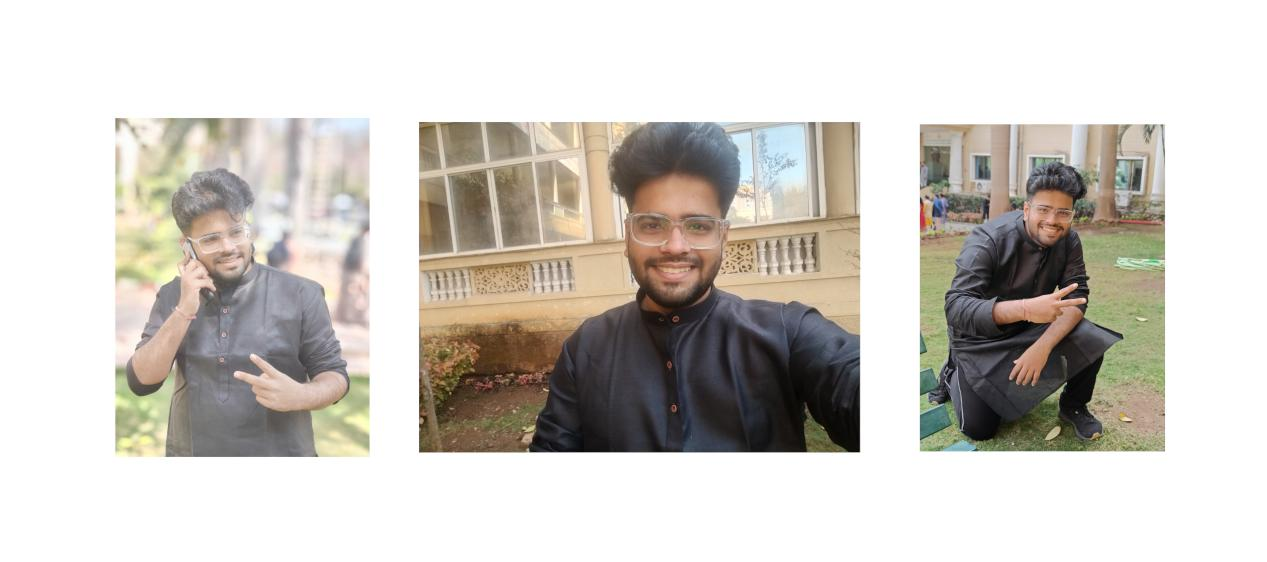
\includegraphics[height=.25\textwidth]{saubhagya.jpg} \\
        \hline
        2                      & Avishkar      & 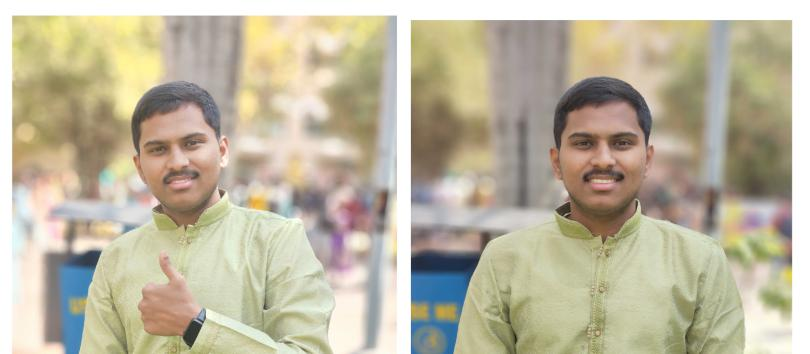
\includegraphics[height=.25\textwidth]{avishkar.jpg}  \\
        \hline
        3                      & Karad         & 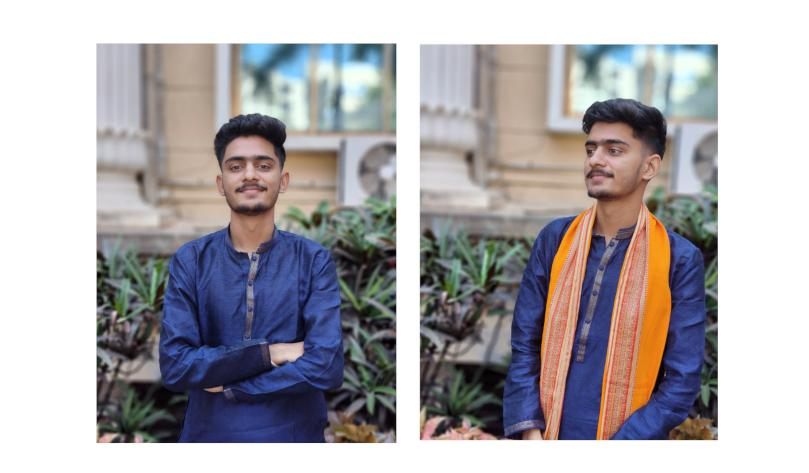
\includegraphics[height=.25\textwidth]{karad.jpg}     \\
        \hline
        4                      & Krish         & 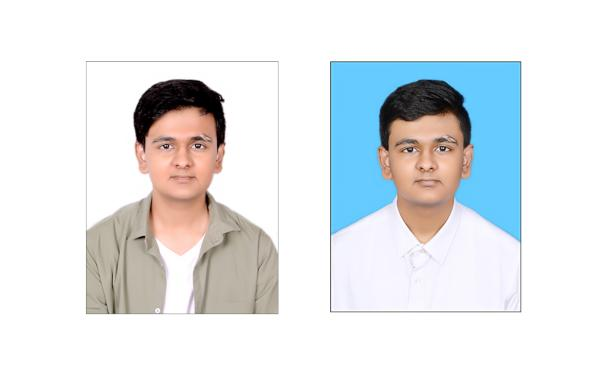
\includegraphics[height=.25\textwidth]{krish.jpg}     \\
        \hline
        5                      & Parth         & 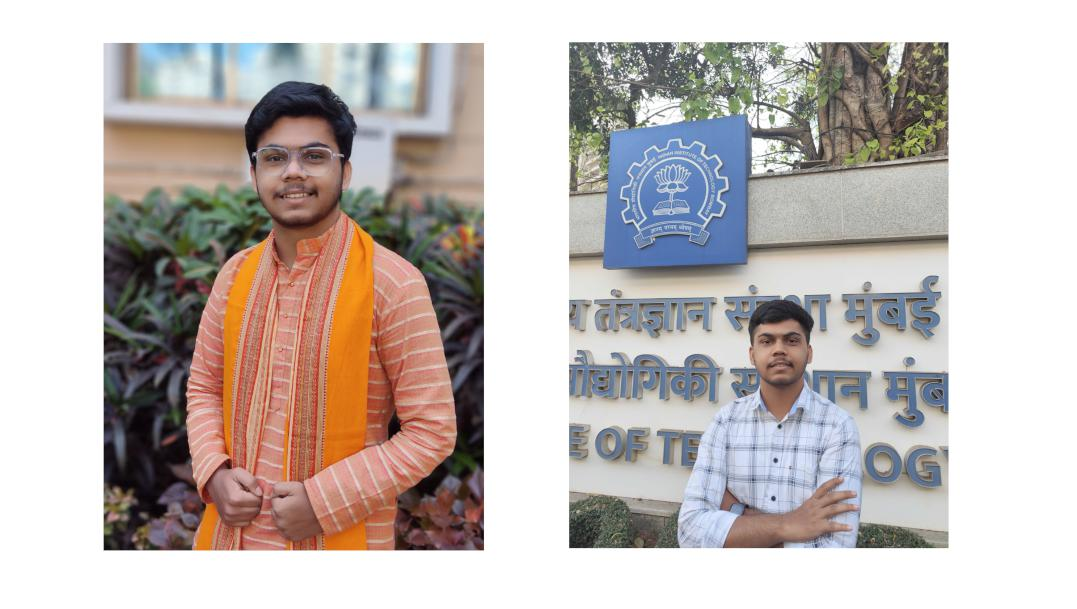
\includegraphics[height=.25\textwidth]{parth.jpg}     \\
        \hline
    \end{tabular}
    \caption{Training Data Images}
\end{table}



\subsection{Creation of Dataset}
\subsubsection{Cropped Faces using openCV-haar-cascades}
The following code generated 18,832 possible faces (245x245px) each. The code uses the OpenCV library to detect faces in images and crop them. The cropped faces are then saved in a specified output folder. The code uses the Haar Cascade classifier for face detection, which is a popular method for real-time face detection. 
\begin{lstlisting}[language=Python]
import cv2
import os
import numpy as np

def detect_and_crop_faces(input_folder, output_folder, padding=10):
    if not os.path.exists(output_folder):
        os.makedirs(output_folder)
    
    face_cascade = cv2.CascadeClassifier(cv2.data.haarcascades + 'haarcascade_frontalface_default.xml')
    
    for filename in os.listdir(input_folder):
        if filename.lower().endswith(('png', 'jpg', 'jpeg', 'webp')):
            image_path = os.path.join(input_folder, filename)
            image = cv2.imread(image_path)
            
            if image is None:
                continue
            
            gray = cv2.cvtColor(image, cv2.COLOR_BGR2GRAY)
            faces = face_cascade.detectMultiScale(gray, scaleFactor=1.1, minNeighbors=5, minSize=(30, 30))
            
            for i, (x, y, w, h) in enumerate(faces):
                x1 = max(x - padding, 0)
                y1 = max(y - padding, 0)
                x2 = min(x + w + padding, image.shape[1])
                y2 = min(y + h + padding, image.shape[0])
                
                face_crop = image[y1:y2, x1:x2]
                output_path = os.path.join(output_folder, f"{os.path.splitext(filename)[0]}_face_{i}.jpg")
                cv2.imwrite(output_path, face_crop)
                print(f"Saved cropped face: {output_path}")

input_folder = os.path.join(os.getcwd(), "input_images")  
output_folder = os.path.join(os.getcwd(), "output_images") 

detect_and_crop_faces(input_folder, output_folder)
    
\end{lstlisting}
Results of the above code are shown in the figure below. The images are cropped and saved in the output folder.

\begin{figure}[H]
    \centering
    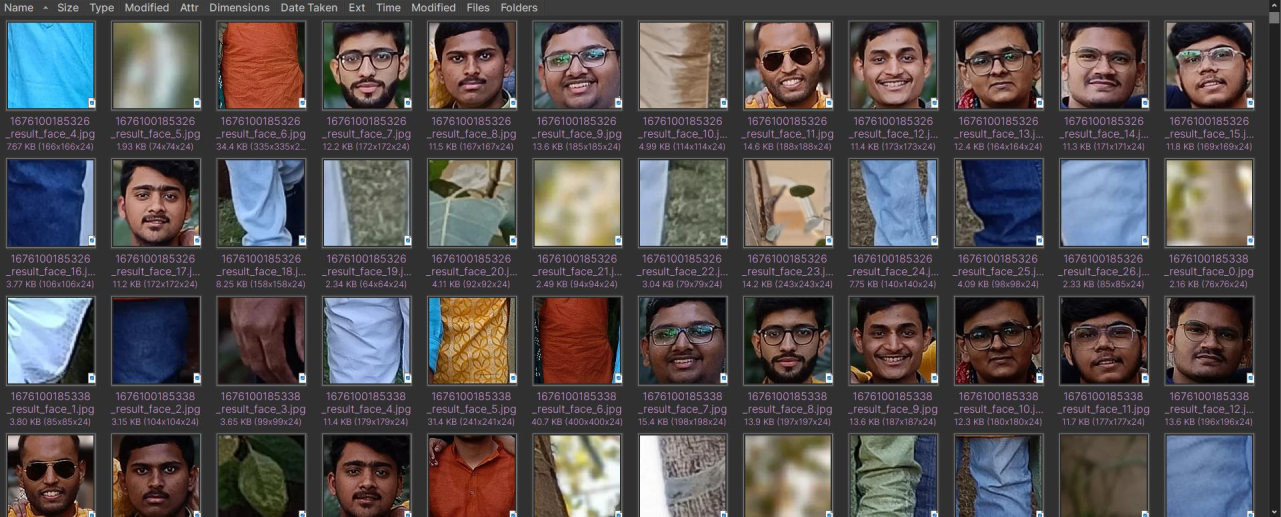
\includegraphics[width=.95\textwidth]{imgs/Cropped images.png}
    \caption{Cropped Faces using OpenCV Haar Cascades}
\end{figure}

\begin{figure}[H]
    \centering
    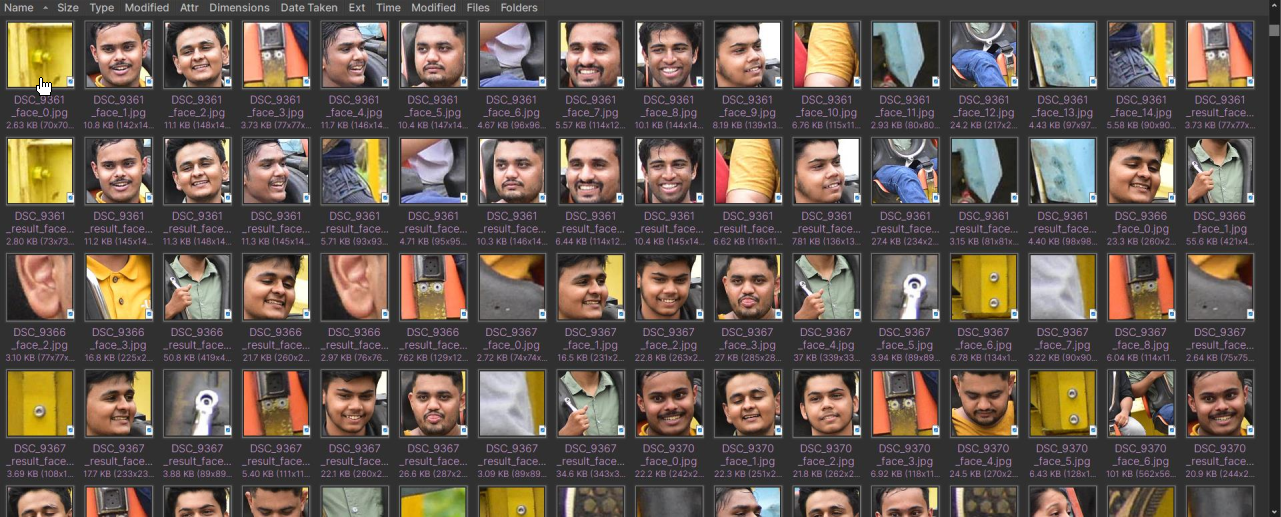
\includegraphics[width=.95\textwidth]{imgs/Copped images 2.png}
    \caption{Cropped Faces using OpenCV Haar Cascades}
\end{figure}

\begin{figure}[H]
    \centering
    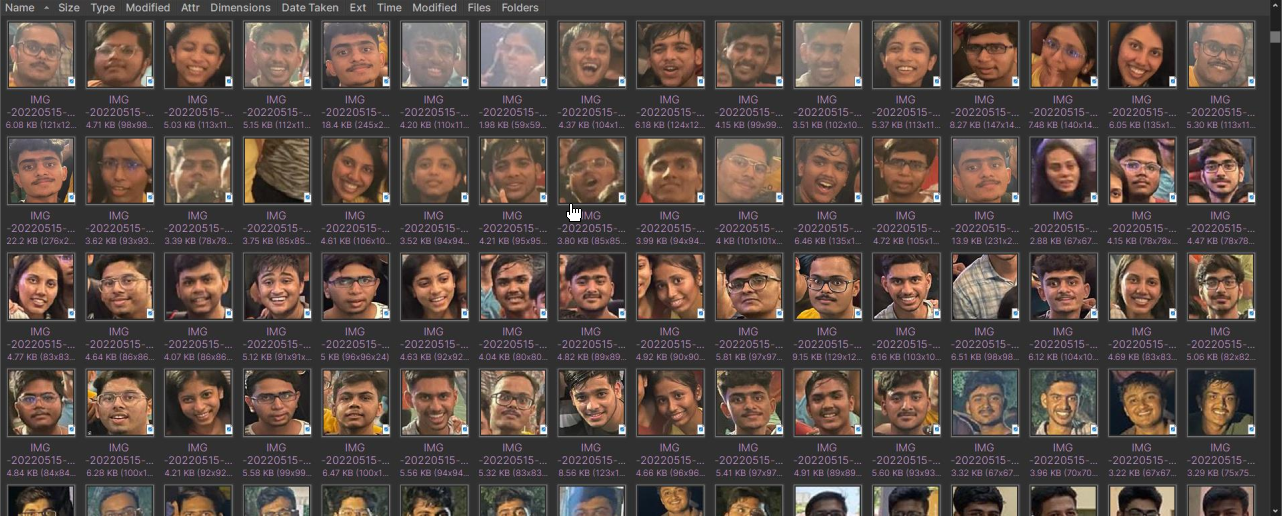
\includegraphics[width=.95\textwidth]{imgs/Copped images 3.png}
    \caption{Cropped Faces using OpenCV Haar Cascades}
\end{figure}

\subsubsection{Manually Segregated photos for 5 people and labelled them}
\begin{figure}[H]
    \centering
    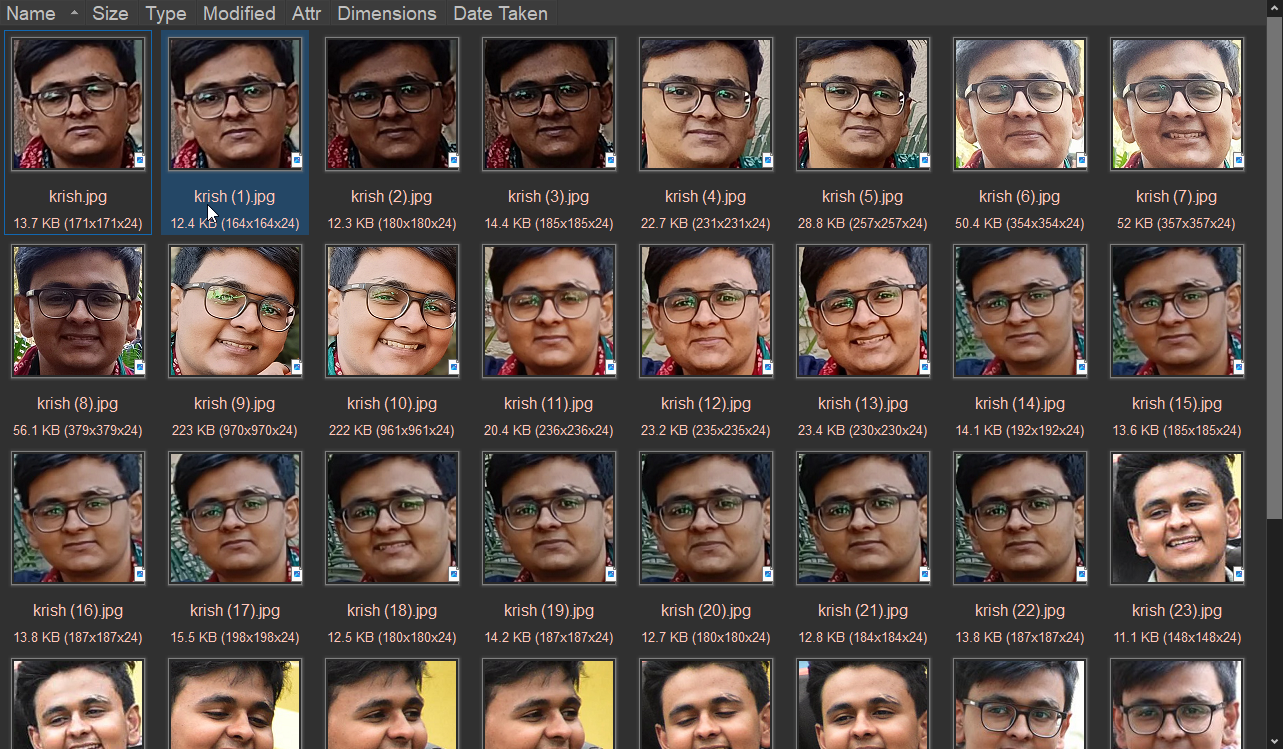
\includegraphics[width=.95\textwidth]{imgs/krishnaraj.png}
    \caption{Krishnaraj's Segregated Images}
\end{figure}
\begin{figure}[H]
    \centering
    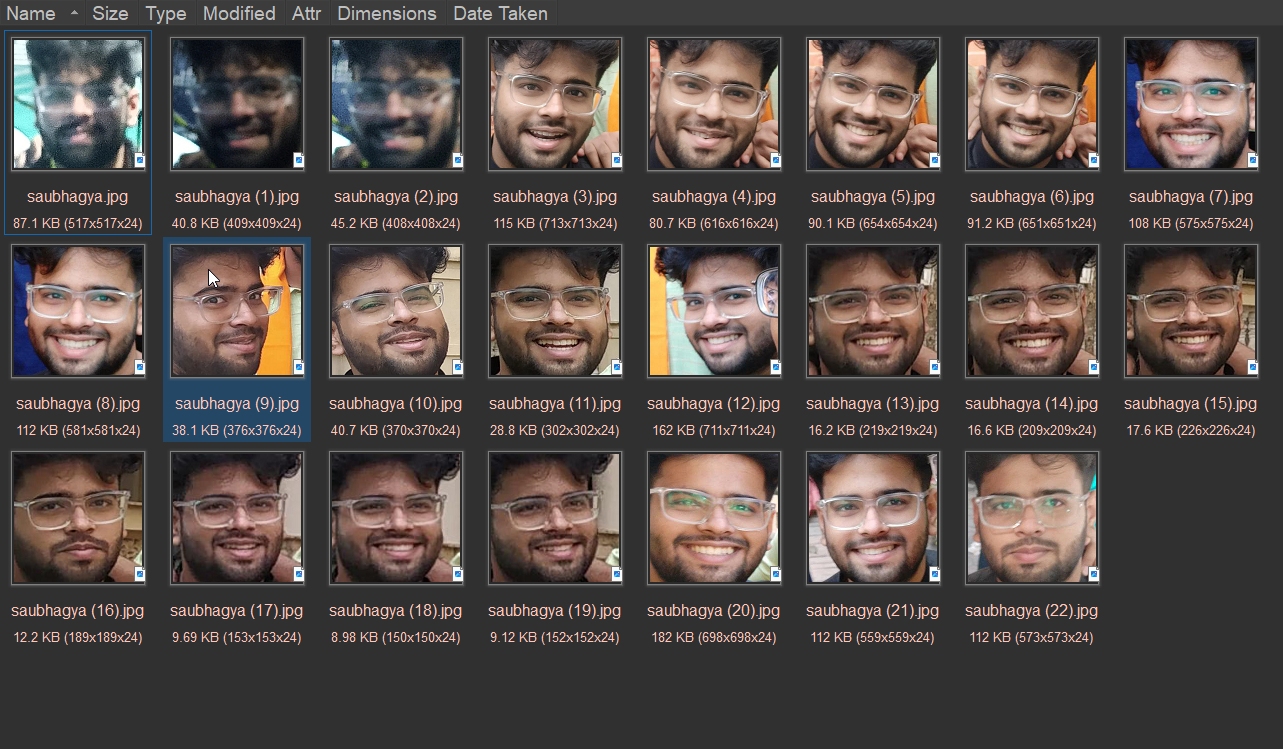
\includegraphics[width=.95\textwidth]{imgs/saubhagya.png}
    \caption{Saubhagya's Segregated Images}
\end{figure}
\begin{figure}[H]
    \centering
    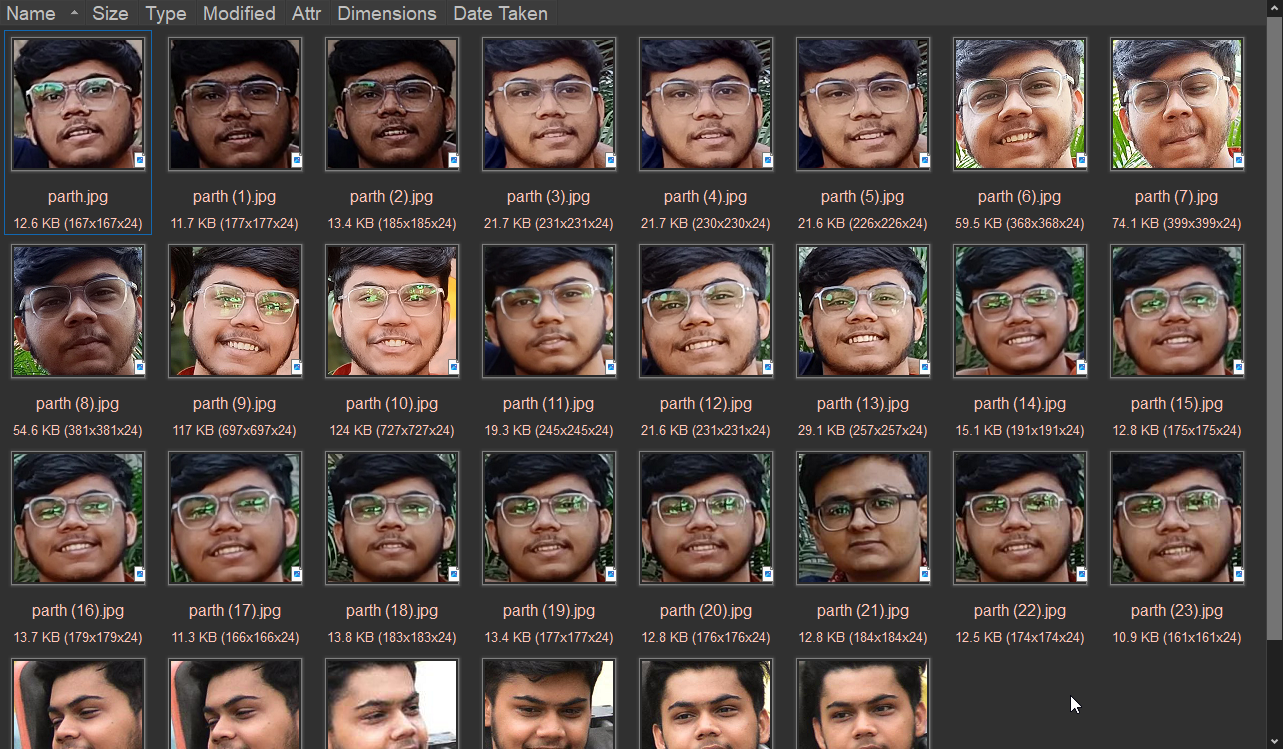
\includegraphics[width=.95\textwidth]{imgs/parth.png}
    \caption{Parth's Segregated Images}
\end{figure}

\begin{figure}[H]
    \centering
    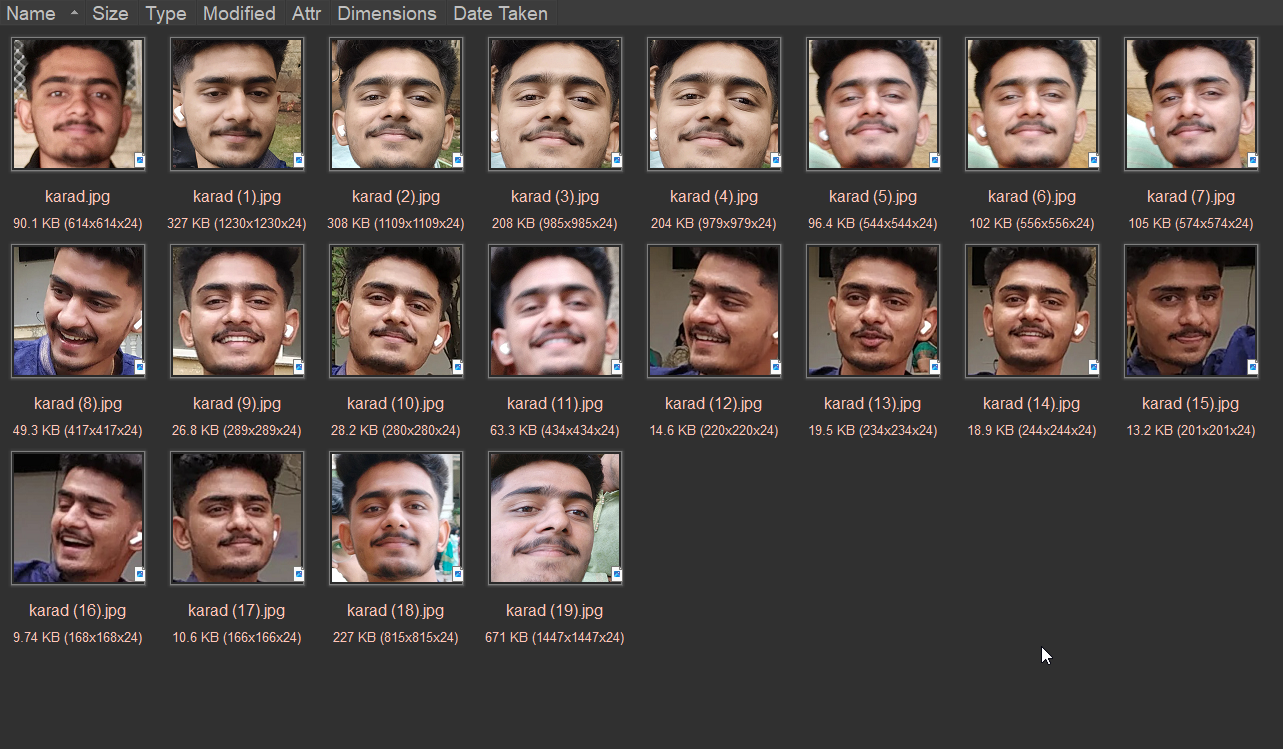
\includegraphics[width=.95\textwidth]{imgs/sourab.png}
    \caption{Sourab's Segregated Images}
\end{figure}

\begin{figure}[H]
    \centering
    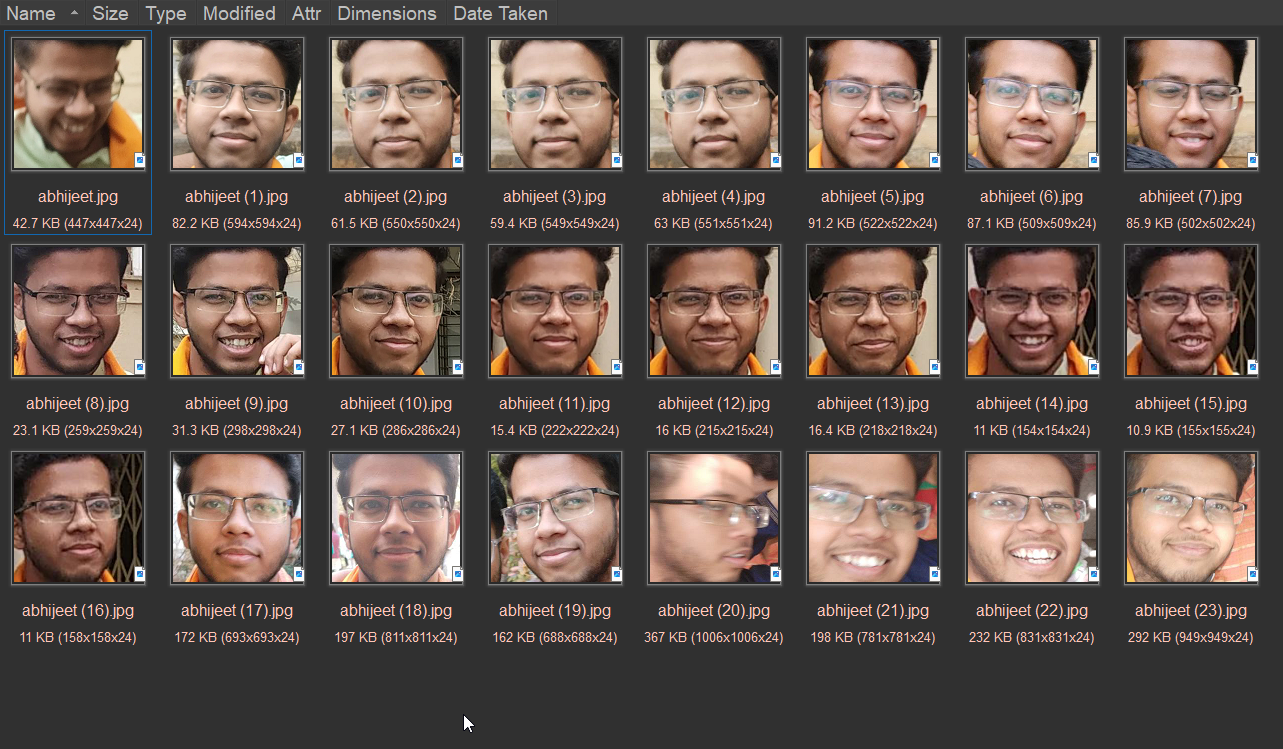
\includegraphics[width=.95\textwidth]{imgs/abhijeet.png}
    \caption{Abhijeet's Segregated Images}
\end{figure}


\subsection{Preliminary Results}
\begin{figure}[H]
    \centering
    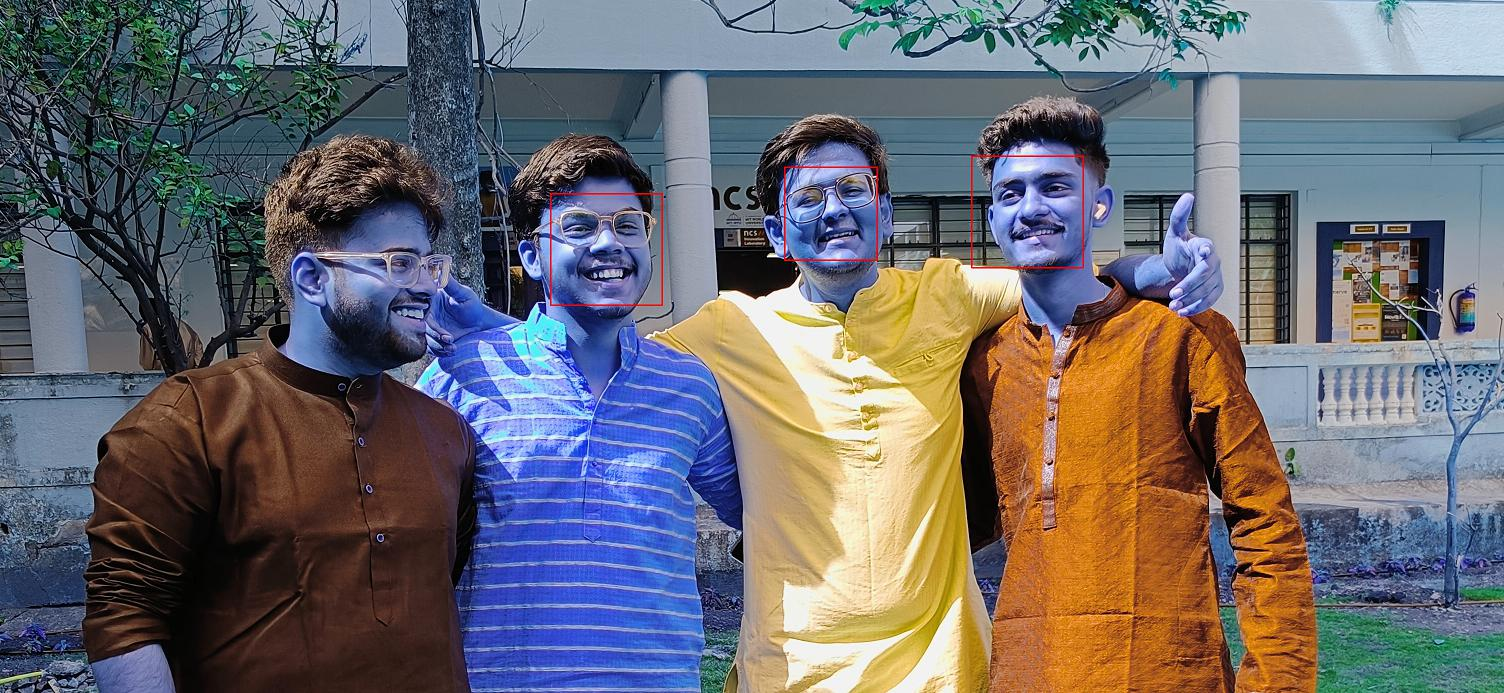
\includegraphics[width=.95\textwidth]{face rec results cropped.jpg}
    \caption{Results identifying 3 of the 4 faces. Empirical results show that the model is working, with accuracy of around 75 \%}
\end{figure}

\subsection{Accuracy per Persion (Class) - LBPH Face Recognizer}
\subsubsection{LBPH Face Recognizer code}
\lstset{language=Python, basicstyle=\ttfamily\small, numbers=left}
\lstinputlisting{code/Module.py}
\begin{figure}[H]
    \centering
    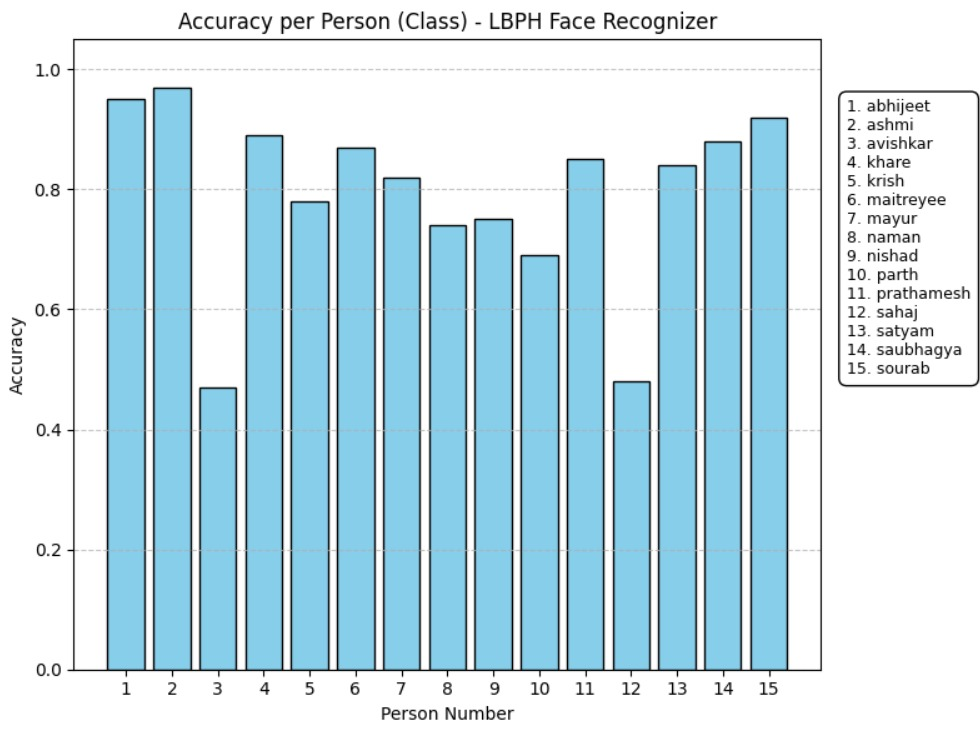
\includegraphics[width=.95\textwidth]{imgs/accuracy per person.jpg}
    \caption{Accuracy per Person (Class) - LBPH Face Recognizer}
\end{figure}


\chapter{Future Prospects for the Attendance Assistant }
Building on our implementation of an automated facial-recognition-based attendance assistant, several avenues can significantly enhance its performance, scalability, and real-world viability:
\section{Integration of advanced Deep-Learning Models}
\begin{itemize}
    \item \textbf{Adopt Lightweight CNNs and Vision Transformers:} Replace or augment traditional feature-based methods (e.g., Eigenfaces, Fisherfaces) with compact convolutional neural networks (MobileNet, EfficientNet) or vision-transformer variants to boost accuracy under varied lighting and poses—while still enabling on-device inference.
    \item \textbf{Hybrid Pipeline Architecture:} Combine fast, classical face detection (e.g., OpenCV Haar cascades) with a secondary deep-learning re-identification stage to balance speed and precision in live classroom or office settings.
\end{itemize}
\section{Dataset Expansion and Synthetic Augmentation}
\begin{itemize}
    \item \textbf{Larger, More Divers Training Sets:} Scale beyond our initial 5-person dataset (=18k crops) by collecting images across multiple sessions, cameras, and demographics to reduce bias and improve generalization.
    \item \textbf{GAN-Based Augmentation:} Leverage generative adversarial networks to synthesize varied facial expressions, occlusions (masks, scarves), and lighting conditions—ensuring robust attendance capture even when subjects wear accessories or move dynamically.
\end{itemize}

\section{Edge Deployment and Resource Optimization}
\begin{itemize}
    \item \textbf{Model Compression Techniques:} Apply quantization and pruning to shrink model size for deployment on low-power edge devices (e.g., Raspberry Pi, embedded IP cameras), minimizing latency in real-time roll-call scenarios.
    \item \textbf{Hardware Acceleration:}Utilize on-board NPUs or Coral TPUs to offload inference, enabling simultaneous multi-camera streams for large lecture halls or multiple office entrances.
\end{itemize}
\section{Privacy, Security, and Ethical Considerations}
\begin{itemize}
    \item \textbf{Federated Learning and on-Device Training:}Implement a federated learning framework so endpoints (e.g., classroom tablets) collaboratively improve the recognition model without sharing raw images—protecting sensitive biometric data by sharing only encrypted weight updates.
    \item \textbf{Anti-Spoofing and liveness Detection:} Integrate texture analysis and micro-motion cues to distinguish live faces from photographs or video replays, safeguarding against presentation attacks
    \item \textbf{Bias Auditing:} Regularly evaluate performance metrics (accuracy, false positives/negatives) across gender, age, and skin-tone strata to identify and mitigate algorithmic bias.
\end{itemize}
\section{Mutlti-Modal and Context-Aware Fusion:}
\begin{itemize}
    \item \textbf{Biometric Fusion:} Biometric Fusion
    Augment facial data with voice recognition or RFID badge readings to confirm identity when face confidence scores drop below a threshold (e.g., under poor lighting).
    \item \textbf{Environmental Sensing:} Dynamically adjust recognition thresholds based on scene context—bright vs. dim classrooms, seated vs. standing students—to maintain both high recall and precision.
\end{itemize}

\section{Broader Applications and Commercialization}
\begin{itemize}
    \item \textbf{Enterprise Time-Tracking Systems:} Extend the attendance assistant to corporate environments, integrating with HR systems for automated timekeeping and employee verification at entrances.
    \item \textbf{Smart-campus and IoT Integration:} Link attendance data with campus access control, library entry logs, and canteen payments to create a unified student experience.
    \item \textbf{Analytics Dashboard:} Offer administrators real-time dashboards showing attendance trends, tardiness patterns, and automated alerts for absenteeism spikes.
\end{itemize}
By pursuing these directions—grounded in our core implementation and the comparative analyses documented earlier—our Attendance Assistant can evolve into a robust, privacy-preserving, and widely deployable solution for both educational institutions and enterprises alike.
\chapter{Conclusion}
In this seminar, we have discussed the various face recognition algorithms and techniques used in the field of computer vision. We have compared the performance of these algorithms based on accuracy, efficiency, and scalability. We have also discussed the advantages and disadvantages of face recognition technology and its applications in real-world scenarios.

\begin{itemize}
    \item Face recognition technology is a powerful biometric technology that can be used for a wide range of applications, from security to personalization.
    \item There are several face recognition algorithms and techniques available, each with its own strengths and weaknesses.
    \item By comparing the performance of different face recognition algorithms and techniques, we can gain insights into their suitability for different applications.
    \item The evaluation metrics provide a quantitative measure of the performance of face recognition algorithms and techniques, helping us identify the most suitable approach for a given application.
    \item Face recognition technology has the potential to revolutionize various industries and improve the quality of life for individuals by providing secure and personalized services.
\end{itemize}
\clearpage
\begin{thebibliography}{10}
    \bibitem{1}
    Paul, Sanmoy and Acharya, Sameer Kumar, A Comparative Study on Facial Recognition Algorithms (December 21, 2020). e-journal - First Pan IIT International Management Conference – 2018, Available at SSRN: https://ssrn.com/abstract=3753064 or http://dx.doi.org/10.2139/ssrn.3753064
    \bibitem{2}
    Kaur, P., Krishan, K., Sharma, S.K. and Kanchan, T., 2020. Facial-recognition algorithms: A literature review. Medicine, Science and the Law, 60(2), pp.131-139.
    \bibitem{3}
    Kukula EP, Elliott SJ. Evaluation of a facial recognition algorithm across three illumination conditions. IEEE Aerospace and Electronic Systems Magazine. 2004 Sep;19(9):19-23.
    \bibitem{4}
    Kukula EP, Elliott SJ. Evaluation of a facial recognition algorithm across three illumination conditions. IEEE Aerospace and Electronic Systems Magazine. 2004 Sep;19(9):19-23.
    \bibitem{5}
    Emami S, Suciu VP. Facial recognition using OpenCV. Journal of Mobile, Embedded and Distributed Systems. 2012 Mar 30;4(1):38-43.
    \bibitem{6}
    Chen J, Jenkins WK. Facial recognition with PCA and machine learning methods. In2017 IEEE 60th international Midwest symposium on circuits and systems (MWSCAS) 2017 Aug 6 (pp. 973-976). IEEE.

    \bibitem{7}
    Schenkel T, Ringhage O, Branding N. A Comparative Study of Facial Recognition Techniques: With focus on low computational power.
    \bibitem{8}
    Paul, S. and Acharya, S.K., 2020, December. A comparative study on facial recognition algorithms. In e-journal-First Pan IIT International Management Conference–2018.
    \bibitem{9}
    Delbiaggio, N., 2017. A comparison of facial recognition’s algorithms.
    \bibitem{10}
    Coe, J. and Atay, M., 2021. Evaluating impact of race in facial recognition across machine learning and deep learning algorithms. Computers, 10(9), p.113.
    \bibitem{11}
    Dirin, Amir, Nicolas Delbiaggio, and Janne Kauttonen. "Comparisons of facial recognition algorithms through a case study application." (2020): 121-133.

\end{thebibliography}

\end{document}
